\chapter{State of the Art}\label{ch:sota}

We divide this chapter into four sections. \hyperref[sec:ch2-sota-generic]{Section} \ref{sec:ch2-sota-generic} presents background knowledge on unsupervised anomaly detection and on Explainable Artificial Intelligence (XAI) related to the work done in this thesis. In \hyperref[subsec:ch2-sota-unsupervised-anomaly-ml]{Subsection} \ref{subsec:ch2-sota-unsupervised-anomaly-ml}, we first introduce the SOTA related to unsupervised anomaly detection through Machine Learning (ML) models. Complementing this, we review some of the main Explainable Artificial Intelligence (XAI) techniques that can be used over an underlying black box model for generating explanations about the model's decision. We review the SOTA of rule extraction techniques in \hyperref[subsec:ch2-sota-xai-rule-extraction]{Subsection} \ref{subsec:ch2-sota-xai-rule-extraction}, and we also analyse novel interpretable ML models that can be used as a surrogate model for generating explanations in \hyperref[subsec:ch2-sota-interpretable-ml]{Subsection} \ref{subsec:ch2-sota-interpretable-ml}. 

Following this, we focus on the current usage of XAI for the specific case of anomaly detection in \hyperref[sec:ch2-sota-xai-anomaly-detection]{Section} \ref{sec:ch2-sota-xai-anomaly-detection}. Also, XAI needs to take into account prior domain knowledge (for the use cases when this is available) in order to provide explanations that are aligned to it. Because of that, we also review in \hyperref[subsec:ch2-domain-knowledge-xai]{Subsection} \ref{subsec:ch2-domain-knowledge-xai} the current SOTA regarding the combination of prior domain knowledge and XAI.

Following this, even though there are several XAI methods that can be used for explaining an unsupervised anomaly detection model, we need some quantitative metrics for comparing the explanations outputs. Thus, previously in \hyperref[sec:ch2-metrics-xai]{Section} \ref{sec:ch2-metrics-xai} we analyse the SOTA regarding XAI metrics for measuring the quality of the explanations. 

Then, since this thesis analyses the usage of XAI with unsupervised anomaly detection models within several real-world use cases, we devote \hyperref[sec:ch2s-sota-specific]{Section} \ref{sec:ch2s-sota-specific} to the analysis of the literature regarding anomaly detection within similar industry cases, regarding network traffic and vehicle fuel consumption. In  \hyperref[subsec:ch2-sota-comms]{Subsection} \ref{subsec:ch2-sota-comms} we present first the analysis for anomaly detection in network traffic. After that, in \hyperref[subsec:ch2-sota-fuel-factors]{Subsection} \ref{subsec:ch2-sota-fuel-factors} we review the prior domain knowledge regarding fuel factors that impact in the fuel consumption of petrol and diesel vehicles. This is complemented with \hyperref[subsec:ch2-sota-ml-fuel-consumption]{Subsection} \ref{subsec:ch2-sota-ml-fuel-consumption}, where we analyze the literature regarding the usage of some of those fuel factors for predicting vehicle fuel consumption with ML. Then, in \hyperref[subsec:ch2-sota-anomaly-fuel]{Subsection} \ref{subsec:ch2-sota-anomaly-fuel}, we review the literature regarding different applications of anomaly detection within vehicle fuel consumption.

Finally, in \hyperref[sec:ch2-sota-summary]{Section} \ref{sec:ch2-sota-summary}, we summarize our literature review, highlighting the specific lines that need further research, which are related to the contributions of this thesis.

\section{Background}\label{sec:ch2-sota-generic}
In this section, we describe the topics of unsupervised anomaly detection, and XAI techniques for model explainability, providing an introduction to XAI, XAI with rule extraction techniques and XAI through interpretable ML models. Regarding the XAI techniques for rule extraction, we divide the subsection into two parts: first, one for model-specific techniques for the case of OneClass Support Vector Machine (OCSVM) algorithm for anomaly detection (since it is one of the algorithms used within this thesis), and one for model-agnostic techniques.

\subsection{Unsupervised ML for anomaly detection}\label{subsec:ch2-sota-unsupervised-anomaly-ml}
The review of \parencite{ruff2021unifying} provides an extensive analysis of the SOTA of ML models for anomaly detection, including unsupervised ones. Unsupervised ML models for anomaly detection can be differentiated according to their feature map, or according to the type of model used (in terms of how the decision frontier is obtained). Regarding the feature map, there are two possible types. First, Shallow models (i.e. Minimum Volume Ellipsoid) versus Deep ones (i.e. Generative Adversarial Networks). Regarding the type of model, four types are mentioned: classification (i.e. OCSVM), probabilistic (i.e. Kernel Density Estimation), reconstruction (i.e. Principal Component Analysis, Deep AutoEncoders) and distance-based (i.e. IsolationForest, Local Outlier Factor). 

OCSVM is a type of Kernel-based One-Class Classification anomaly detection model that is well-suited for multimodal, nonlinear and nonconvex data sets. OCSVM is also an algorithm that, since its original formulation \parencite{scholkopf2000support}, has being developed with many variations.

OCSVM has advantages in terms of computational performance \parencite{wang2004anomaly}. One of the reasons is that it creates a decision frontier using only the support vectors (like general supervised SVM). Another advantage is that model training always leads to the same solution because the optimization problem is a convex one. However, SVM (hence OCSVM) algorithms are difficult to explain due to the mathematically-complex method that obtains the decision frontier \parencite{arrieta2020explainable}.

From a theoretical point of view, Support Vector Machines (SVM) for classification maps the data points available in the data set to a higher dimensional space than the one determined by their features, so that the separation among classes may be done linearly. It uses a hyperplane obtained from data points from all of the classes. These data points, known as support vectors, are the ones that are closer to each other and the only ones needed to determine the decision frontier. However, it is not really necessary to map to a higher dimension due to the fact that the equation that appears in the optimization of the algorithm uses a dot product of those mapped points. Because of that, the only thing to be calculated is such dot product, something that can be accomplished with the well-known kernel trick. Hence instead of calculating explicitly the mapping to a higher dimension the equation is solved using a kernel function. 

In OCSVM there are no labels. Hence all data points are considered to belong to a same class at the beginning. The decision frontier is computed trying to separate the region of the hyperspace with a higher number of data points close to each other from another that has small density, considering those points as anomalies. To do so the algorithm tries to define a decision frontier that maximizes the distance to the origin of the hyperspace and that at the same time separates from it the maximum number of data points. This compromise between those factors leads to the optimization of the algorithm and allows obtaining the optimal decision frontier. Those data points that are separated are labeled as non-anomalous (+1) and the others are labeled as anomalous (-1).

The optimization problem is reflected in the following equations:
\begin{equation}\label{eq:c2-sota-eq1}
\begin{split}
  min_{w, \xi_i, \rho} = \frac{1}{2} ||w||^2 + \frac{1}{\nu n}\sum_{i=1}^{n}(\xi_i - \rho) \\
  \text{subject to:}\\
  (w, \phi(x_i)) \geq \rho - \xi_i\:\:for\:i = 1,...,n  \\
  \xi_i \geq 0\:\:for\:i = 1,...,n
\end{split}
\end{equation}

In \hyperref[eq:c2-sota-eq1]{Equation} \ref{eq:c2-sota-eq1}, $\nu$ is a hyper-parameter known as \textit{rejection rate}, which needs to be selected by the user. It sets an upper bound on the fraction of anomalies that can be considered, and also defines a lower bound on the fraction of support vectors that can be considered. The rest of the variables are: $w$ is the normal vector to the hyperplane, $\rho$ is a constant, $x_i$ a data point, $\phi(x_i)$ the feature map, $\xi_i$ is a slack variable and $n$ the number of observations.

Using Lagrange techniques, the decision frontier obtained is the following one:
\begin{equation} \label{eq:ch2-sota-eq2}
\begin{split}
f(x) = sgn((w, \phi(x_i) - \rho) \Rightarrow \\
f(x) = sgn(\sum_{i=i}^{n}\alpha_i K(x_i,x) - \rho)
\end{split}
\end{equation}

Where $K(x_i,x)$ is the kernel. Hence the hyper-parameters that must be defined in this method are the rejection rate, $\nu$, and the type of kernel used. 

\subsection{Explainable Artificial Intelligence}\label{subsec:ch2-sota-intro-xai}
Even though unsupervised ML algorithms in general, and OCSVM in particular, are useful for detecting anomalies by finding complex decision functions, one issue is that they do not provide direct insights about the reasons behind their decision. This is exemplified in  \hyperref[fig:XAItradeoff]{Figure} \ref{fig:XAItradeoff}, where we see the trade-off between model's intepretability and accuracy, highlighting that complex models (such as SVM) that provide high levels of accuracy, sacrifice interpretability in exchange. 

\begin{figure}[h!]
\centering
 \begin{tabular}{c@{\qquad}c@{\qquad}c}
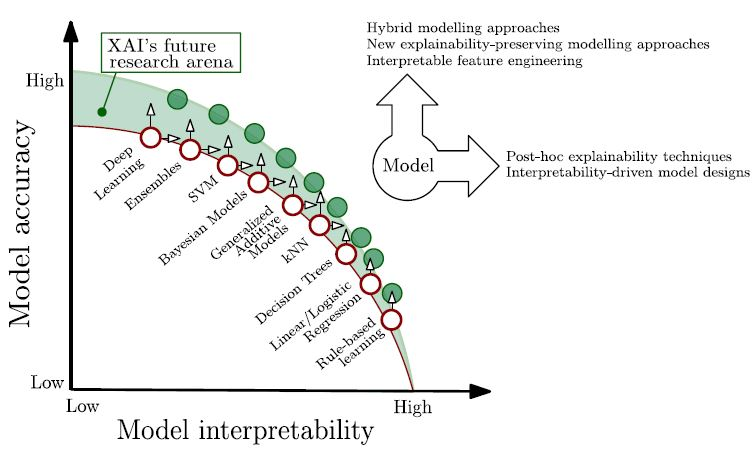
\includegraphics[width=0.8\columnwidth]{figures/XAI_tradeoff.jpg}
  \end{tabular} 
  \caption{Trade-off between model interpretability and model performance \parencite{arrieta2020explainable}.\label{fig:XAItradeoff}}
\end{figure}

Thus, the dichotomy would be between choosing models that provide information about their decisions (known as whitebox models, like a linear regression algorithm), or choosing highly accurate ones that are opaque in that regard (known as blackbox models, like SVM). For many domains, a simple whitebox model may suffice, so both high accuracy and high interpretability are obtained. However, for other more complex domains, high accuracy may only be attainable through blackbox models, thus losing the intepretability information. XAI comes to close the bridge in this dichotomy, providing an additional layer that extracts information about the model's decision. Thus, even if the model is not intepretable by itself, XAI can generate explanations about its decision \parencite{arrieta2020explainable}. 

There are several approaches that can be considered for generating these explanations with XAI. This is something addressed within XAI taxonomies, which classify methods according to different aspects. One of them is related to whether the XAI technique uses specific information that is only available to some blackbox models (model specific), or by contrast, it considers the blackbox model as an "oracle" and infers information about its decision process by analysing its inputs and/or outputs only (model agnositc). An example of the former would be a XAI technique for SVM that uses the information about the support vectors (SV). SV are only available for SVM techniques, and do not exist within other ML algorithms. Thus, the XAI technique only works for a subset of ML algorithms. By contrast, model agnostic techniques could be theoretically be applied to any ML model. This idea is shown in \hyperref[fig:XAIspecificVSagnostic]{Figure} \ref{fig:XAIspecificVSagnostic}.
 
\begin{figure}[h!]
\centering
 \begin{tabular}{c@{\qquad}c@{\qquad}c}
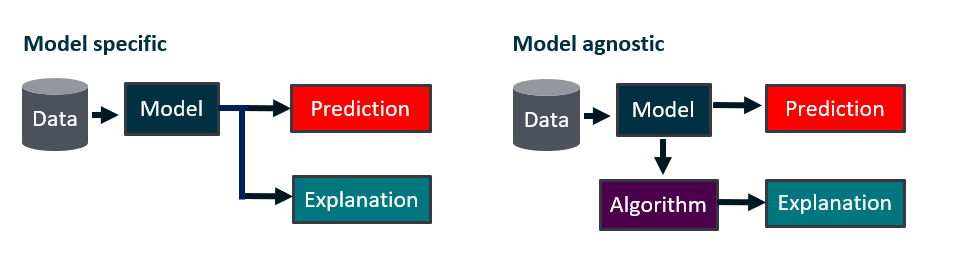
\includegraphics[width=0.8\columnwidth]{figures/XAI_specific_vs_agnostic.PNG}
  \end{tabular} 
  \caption{XAI taxonomy: classifying methods depending on whether they are model specific or model agnostic.\label{fig:XAIspecificVSagnostic}}
\end{figure}

There are other aspects that can be considered for classifying XAI techniques. One of them is the output of the techniques. The XAI technique could be explaining only a specific model prediction (local explanations) or could be explaining the whole decision frontier of the model (global explanations). Also, the explanations could be provided in terms of feature relevance, or could be provided as rule-based explanations \parencite{arrieta2020explainable}. An example of these aspects is shown in \hyperref[fig:XAIapproaches]{Figure} \ref{fig:XAIapproaches}.

\begin{figure}[h!]
\centering
 \begin{tabular}{c@{\qquad}c@{\qquad}c}
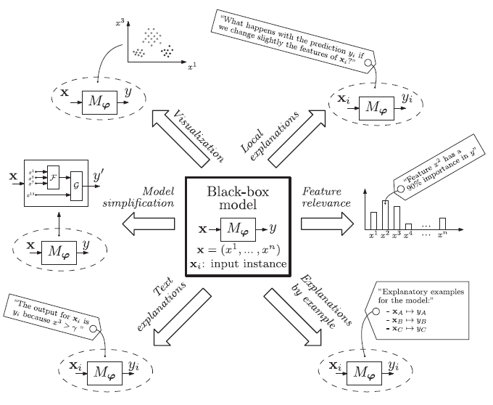
\includegraphics[width=0.6\columnwidth]{figures/XAI_Approaches.PNG}
  \end{tabular} 
  \caption{XAI taxonomy: classifying methods according to their output. \parencite{arrieta2020explainable}\label{fig:XAIapproaches}}
\end{figure}

Finally, beyond the aforementioned taxonomies, there are other important aspects to consider within XAI. Formally, XAI can be defined as "\textit{given an audience, an explainable Artificial Intelligence is one that produces details or reasons to make its functioning clear or easy to understand}" \parencite{arrieta2020explainable}. Thus, XAI must consider not only the underlying model's information, but also the target audience that will receive the explanations. Because of that, XAI is not the same as model intepretability, since the former deals with an active characteristic, while the latter talks about a passive property available to whitebox models only. There are different audiences that can be considered, as shown in \hyperref[fig:XAIaudience]{Figure} \ref{fig:XAIaudience}.

\begin{figure}[h!]
\centering
 \begin{tabular}{c@{\qquad}c@{\qquad}c}
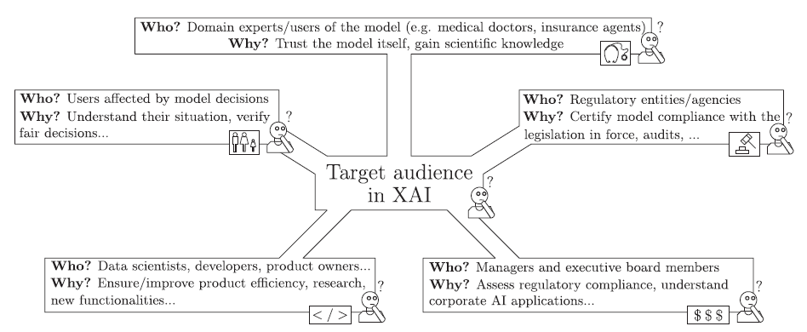
\includegraphics[width=0.8\columnwidth]{figures/XAI_audience.png}
  \end{tabular} 
  \caption{Different types of XAI audiences. \parencite{arrieta2020explainable}\label{fig:XAIaudience}}
\end{figure}


\subsection{Rule extraction techniques in XAI}\label{subsec:ch2-sota-xai-rule-extraction}
As mentioned in the previous subsection, rule extraction methods are a type of post-hoc XAI techniques that have in common that they provide rule-based explanations  \parencite{arrieta2020explainable}. This is exemplified in \hyperref[fig:RuleExtractionExamples]{Figure} \ref{fig:RuleExtractionExamples}, where we see different outputs for rule extraction methods with the case of Decision Trees or rule-based approaches with IF-ELSE rules.

\begin{figure}[h!]
\centering
 \begin{tabular}{c@{\qquad}c@{\qquad}c}
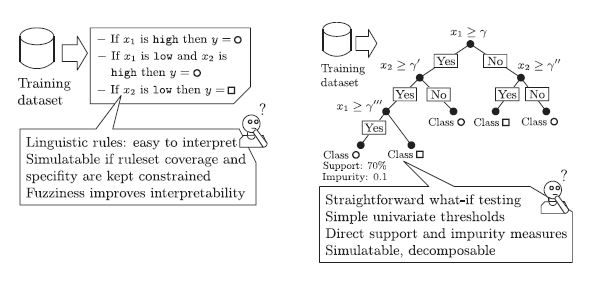
\includegraphics[width=0.8\columnwidth]{figures/RuleExtractionExamples.JPG}
  \end{tabular} 
  \caption{Different examples of rule extraction approaches: through Decision Trees or IF-ELSE rules \parencite{arrieta2020explainable}.\label{fig:RuleExtractionExamples}}
\end{figure}

Beyond that, rule extraction techniques could be classified within any other XAI taxonomy aspect: they can be model agnostic or model specific, or they can provide local and/or global explanations. Within this subsection, we focus on describing different rule extraction techniques depending on whether they are model specific or model agnostic, indicating when these techniques can be used for either global or local explanations (or both).

\subsubsection{Model specific rule extraction techniques in XAI for SVM}\label{subsubsec:ch2-sota-xai-rule-extraction-specific}
\leavevmode\newline
\parencite{barakat2010rule} offers a review of rule extraction techniques for SVM. Focusing on model specific techniques, they highlight three different types of algorithms. The first of them are rule extraction algorithms that use the support vectors from the original model as an input source for generating the rules. This is the case of SQRex-SVM \parencite{barakat2007rule} where the authors propose the usage of a subset of the support vectors for inferring the rules with the usage of a modified sequential covering algorithm. 
The second type of algorithms use both information from the support vectors together with information from the separating hyper-plane. This is the case of RulExSVM \parencite{fu2004extracting}, where the authors propose a technique applicable for SVM with a Radial Basis Function (RBF) kernel. The algorithm uses the support vectors in order to build hyper-rectangles that intersect with the separating hyper-plane. Finally, the last type of techniques use the support vectors, the separating hyper-plane, and the training data. The training data is used to define the regions in the hyperspace, and the support vectors and the hyper-plane define the size of those regions. Within this category appears the proposal of \parencite{nunez2002rule}, which can provide explanations for the whole decision frontier (global), as well as for specific data points (local). We will focus on this last approach since it is the most complete one due to the fact that it uses all the available information for generating the explanations. Their proposal also offers one of the greatest levels of accuracy and fidelity when evaluated over several data sets compared to other proposals.

In \parencite{nunez2002rule}, authors propose a technique called SVM+ Prototypes that can be considered model-agnostic or model specific depending on how is implemented. The general intuition consists in finding hypercubes (or hyperspheres) using the centroids (or prototypes) of data points of each class. Then, it can use as vertices either the support vectors from the SVM model, or the data points from that hyperspace area farther away from that centroid. For the first alternative, the proposal is model specific, since it focuses on a specific component of the model itself (the support vectors). The second one is model-agnostic, since it does not use any information that is specific only for SVM models.
After this, it infers a rule from the values of the vertices of the hypercube that contain the limits of all the points inside it, creating one rule for each hypercube.

For example, a data set that contains two numerical features X and Y will be defined in a 2-dimensional space. The algorithm will create a square that contains the data points on each of the classes, as shown in \hyperref[fig:ch2-sota-outlier0]{Figure} \ref{fig:ch2-sota-outlier0}. The rule that justifies that a data point belongs to class 2 is:
\begin{itemize}
%    \setlength{\itemindent}{2em}
    \item Rule 1: CLASS 2 IF X$\geq$X1 $\land$ Y$\geq$Y1 $\land$ X$\leq$X2 $\land$ Y$\leq$Y2
\end{itemize}

\begin{figure}[h!]
\centering
 \begin{tabular}{c@{\qquad}c@{\qquad}c}
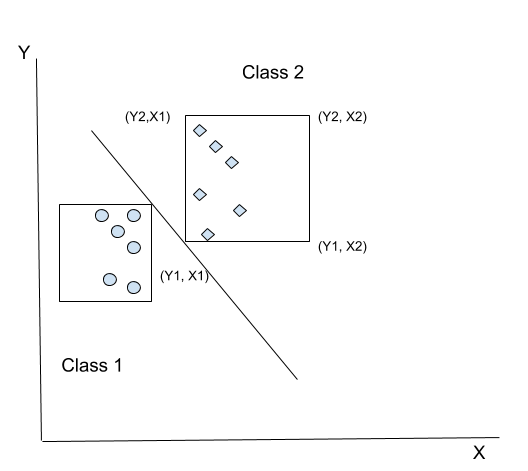
\includegraphics[width=0.5\columnwidth]{figures/outlier_00.png}
  \end{tabular} 
  \caption{SVM with linear kernel classifying data points of two classes.\label{fig:ch2-sota-outlier0}}
\end{figure}

The generated hypercubes may wrongly include points from the other class when the decision frontier is not linear or spherical, as shown in \hyperref[fig:ch2-sota-outlier1]{Figure} \ref{fig:ch2-sota-outlier1}. In this case, the algorithm considers an additional number of clusters trying to include the points into a smaller hypercube, as shown in \hyperref[fig:ch2-sota-outlier2]{Figure} \ref{fig:ch2-sota-outlier2}.

\begin{figure}[h!]
\centering
  \begin{tabular}{c@{\qquad}c@{\qquad}c}
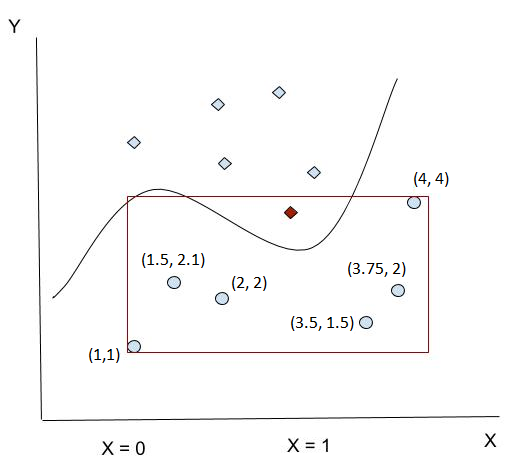
\includegraphics[width=0.5\columnwidth]{figures/outlier_01.png}
  \end{tabular} 
  \caption{A hypercube generated using the farthest points leads to the wrong inclusion of data from the another class.\label{fig:ch2-sota-outlier1}}
\end{figure}

\begin{figure}[!h]
\centering
  \begin{tabular}{c@{\qquad}c@{\qquad}c}
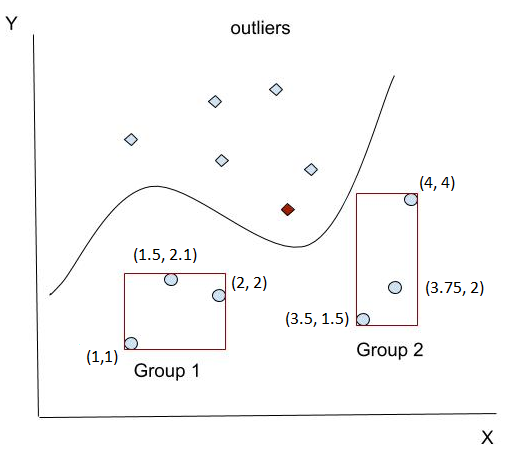
\includegraphics[width=0.5\columnwidth]{figures/outlier_02.png}
  \end{tabular} 
  \caption{Using more hypercubes avoids the aforementioned problem. Now there is no wrong inclusion of data points from another class.\label{fig:ch2-sota-outlier2}}
\end{figure}

A rule will be generated for each hypercube, considering all those scenarios as independent, leading to this output:
\begin{itemize}
    \setlength{\itemindent}{2em}
    \item Group 1: CLASS 1 IF X $\geq$ 1 $\land$ X $\leq$ 2 $\land$ Y $\geq$ 1 $\land$ Y $\leq$ 2.1\
    \item Group 2: CLASS 1 IF X $\geq$ 3.5 $\land$ X $\leq$ 4 $\land$ Y $\geq$ 1.5 $\land$ Y $\leq$ 4
\end{itemize}

There are some downsides of that method in supervised tasks, especially when the problem is not simply a binary classification or when the algorithm is performing a regression. For instance, the number of rules may grow immensely due to the fact that a set of rules will be generated for each category and each set may contain a huge number of rule groups, leading to an output that may be difficult to understand by humans.

However, in OCSVM these difficulties may be potentially mitigated due to two reasons. On the one hand, the explanations are reduced to rules that explain when a data point is not an anomaly (so there would be no need to define rules for the anomalies). On the other hand, the algorithm tries to group all non-anomalous points together, setting them apart from the outliers. Because of this, the chance to define a hypercube that does not contain a point from the another class may be higher than in a standard classification task. Both the unbalanced inherent nature of data points in anomaly detection (few anomalies vs. many more non-anomalous data points) and the fact that non-anomalous points tend to be closer to each other may help achieving good results with this method.

\subsubsection{Model-agnostic rule extraction techniques in XAI}\label{subsubsec:ch2-sota-xai-rule-extraction-agnostic}
\leavevmode\newline
% Some examples
Many rule extraction proposals contribute to XAI without the need to use any specific information from a particular type of model \parencite{arrieta2020explainable}. The only information necessary for building the rules is the input features and the model outputs. Some techniques use all the training data, while others need only a few input instances, or they can even generate artificial data points to infer the decision frontier. An example of this last approach is the LIME (Local Interpretable Model-agnostic Explanations) algorithm \parencite{ribeiro2016should}, where random samples are generated in order to train a linear model that approximates a complex decision function around a specific data point. Following the taxonomy of \parencite{arrieta2020explainable}, model-agnostic techniques through rule-based approaches can be used both for global and for local explanations, as shown in \hyperref[fig:ModelAgnosticDiagram]{Figure} \ref{fig:ModelAgnosticDiagram}.

\begin{figure}[h!]
\centering
 \begin{tabular}{c@{\qquad}c@{\qquad}c}
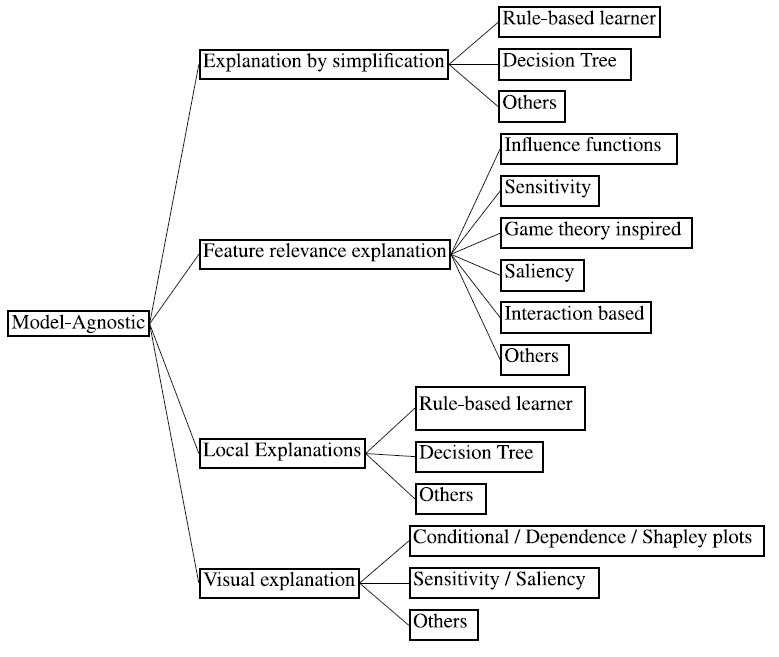
\includegraphics[width=0.7\columnwidth]{figures/ModelAgnosticDiagram.PNG}
  \end{tabular} 
  \caption{Taxonomy for model agnostic XAI techniques, where rule-based approaches appear both for local and global explanations within the case of Decision Trees and Rule-based learners. \parencite{arrieta2020explainable}.\label{fig:ModelAgnosticDiagram}}
\end{figure}

These techniques were initially conceived for supervised ML. However, they can be extended for unsupervised ML for anomaly detection, since their output is analogous to a binary classifier where the classes are heavily imbalanced.

% Surrogate DT
A general way to approximate any blackbox model globally is by using a surrogate supervised decision model trained over the same data set, but instead of using the real labels (the ones used for the blackbox model), it is trained over the predictions of that blackbox model \parencite{molnar2019interpretable}. This may be accomplished with any ML model, but it is useful to do it with a whitebox model that can be directly interpreted by humans. An example is a Decision Tree (DT) model, as indicated in \hyperref[fig:ModelAgnosticDiagram]{Figure} \ref{fig:ModelAgnosticDiagram}. DT allows explaining the classification logic of the blackbox model through the usage of rules, which can be used even for classifying new instances. The advantages of using a DT as a surrogate global model is its flexibility (it can be applied over any model in an agnostic way) and simplicity (it is a solution that is easy to explain). However, this approximation at the end leads to explain a proxy model, and not the actual data, since the surrogate model never sees the true target values.

\hyperref[fig:ModelAgnosticDiagram]{Figure} \ref{fig:ModelAgnosticDiagram} also shows a category of rule-based techniques known as rule-based learners. In many cases, these techniques can be used for both global and local explanations. Following this, we will describe five methods within this category: RuleFit, SkopeRules, Falling Rule Lists, Boolean Decision Rules via Column Generation, and Generalized Linear Rule Models.

% RuleFit
RuleFit \parencite{friedman2008predictive} is a model-agnostic surrogate model that learns a linear regression model (Lasso regression) that uses as features both the original features of the model, as well as new generated features that represent decision rules. In order to accomplish that, first, a tree model is trained over the output and the input features, and the decision paths between the tree levels are turned into decision rules, except for the ones that lead to the leaf nodes, which are not considered. These rules are used as additional features, along with the original ones, on the Lasso surrogate model. Thanks to this, RuleFit yields both rules as well as their contribution, measured through the coefficients of the Lasso model. In summary, RuleFit generates a white-box model that includes rules as features, that can be interpreted as a standard linear regression one. The only caveat is that, for the original coefficients, the predicted outcome changes by $|\beta_j$ if feature $x_j$ changes by one unit if the other features remain unchanged, while for a feature-rule $r_k$ it is different; if all the conditions of the feature $r_k$ are met, the predicted outcome changes by $\alpha_k$ (the weight associated to that rule-coefficient) for regression. Similarly, for classification tasks, when the conditions of $r_k$ are met, the odds for event vs. no-event changes by a factor of $\alpha_k$.

% SkopeRules
Similarly to RuleFit, SkopeRules \parencite{molnar2019interpretable} is another way to generate rules from tree ensembling techniques. They differ, however, in how they obtain the rules. 
First, SkopeRules generates the rules using surrogate tree ensembles trained using the input features and the target variable. Then, it applies a filtering step in which, using a threshold for Precision and Recall, some rules are removed and some are kept. This step allows selecting only high-performing rules, and removing the ones that do not yield good results. The last step is known as "semantic rule duplication". This step eliminates duplicate rules (rules that are the same or very similar to other ones). It also eliminates again low-performing rules based on their results for a F1-metric. This allows obtaining high-performing as well as heterogeneous rules. The final set of rules is the output of SkopeRules, differing from RuleFit because it does not use a Lasso model to aggregate all rules.

% Bayesian Falling Rule List
Falling Rule Lists (FRL) \parencite{wang2015falling} are classification models that generate a sorted list of IF-THEN rules, thus, they can serve as a model-agnostic global post-hoc rule extraction technique. The rules are binary, and are looked one after the other, in order to see if a particular data point can be classified into one of the classes. The rules are sorted according to the probability of classifying a data point into that class using that rule. Due to that, FRL offers a list of IF-ELSE IF rules associated to a particular class with a decreasing probability score. 

% BooleanRuleCG
Boolean Decision Rules via Column Generation (BRCG) \parencite{NIPS2018_7716} also provides a binary classifier by using disjuntive normal form (DNF, OR-of-ANDs) or conjuntive normal form (CNF, AND-of-ORs) through interpretable rules. In case of DNF, they provide an unordered set of decision rules that classify a data point into the positive category if at least one of the rules is satisfied. This is different than other methods already mentioned, such as BFRL where the rules are ordered in an IF-THEN schema, or the surrogate DT model, that provides the rules in a tree structure schema.

% Generalized Linear Rule Models
Generalized Linear Rule Models (GLRM) \parencite{pmlr-v97-wei19a} generate decision rules and combine within a linear model (generalized additive model, GAM). Thus, they provide both a non-linear modelling, thanks to the decision rules, while keeping the interpretability by using a linear model that ensembles them. However, as \parencite{arya2019one} notice, while it is feasible to interpret linear combinations of rules, if the number of rules increases too much, there is a risk of losing the interpretability of the model. The authors highlight that in order to reduce the rules generated and not lose interpretability, they use a rule selection technique based on column generation (CG). CG searches the spaces of rules and generates them only when they are needed, and then fits again the GLM model. This allows analysing again old rules, re-weight them, and discard the ones that are not needed anymore. This is different to other methods used in the literature, mainly pre-selecting a subset of candidate rules using optimization techniques, or a greedy optimization approach by adding rules one by one using sequential covering or boosting techniques.

% Anchors
Within \hyperref[fig:ModelAgnosticDiagram]{Figure} \ref{fig:ModelAgnosticDiagram} there are also other rule-based learner techniques that can only provide local explanations, like Anchors \parencite{ribeiro2018anchors}. The purpose of Anchors is finding a decision rule that approximates the decision function of the blackbox model around that individual data point. This rule "anchors" the prediction of that data point, so that any perturbation of the features of that point that are still inside the rule will always return the same output from the blackbox model. The approach is as follows. First, the algorithm generates candidate rules that may explain the data point. Then, it evaluates those candidate rules. In order to do that, Anchors generates permutations around the data point (similar data points to the original one) that yield the same result. The result is evaluated by calling the blackbox model (the oracle) and obtaining the classification for that data point. In order to optimize the exploration-exploitation of generating and evaluating data points, it uses a reinforcement learning approach with a Multi-Armed Bandit (MAB) approximation. In this MAB, each arm of the Bandit problem is a candidate rule, and the data points generated, after obtaining their classification result from the blackbox model, are used to compute a precision metric used to evaluate the candidate rule's payoff. This reinforcement learning approach helps minimizing the number of calls to the model in order to reduce the computational cost of the algorithm. Among all the candidate rules, the algorithm then checks if the best one of them matches a predefined convergence criteria. To do that, it filters rules according to a precision threshold, and selects form the remaining ones the one with highest coverage. That rule is used to explain that original data point. If there are no rules that match the convergence criteria, then the algorithm keeps iterating (using a beam search approach) using the B best rules from the previous step in order to generate new candidate rules for the following one. In those following steps, Anchors keep extending the rules with more features (in the first step, it only uses one feature per candidate rule).
Thus, Anchors offers a model-agnostic approach that generate IF-THEN rules, easy to interpret, that are generated in an efficient way thanks to the usage of reinforcement learning (MAB) that can be parallelised. However, Anchors is very sensitive to its initial configuration, like many permutation approach algorithms, such as LIME \parencite{ribeiro2016should}. Another important consideration of Anchors is that, while it keeps the calls to the oracle to a minimum (thanks to MAB), it still requires a lot of calls, and that can affect the runtime of the algorithm.

\subsection{Interpretable Machine Learning models}\label{subsec:ch2-sota-interpretable-ml}
Feature relevance-based explanations techniques \parencite{molnar2019interpretable, arrieta2020explainable} quantify the individual contribution of each training feature to the target variable. This type of explanations can be provided either by post-hoc XAI techniques applied to any type of regression or classification ML model, or by using an interpretable ML model alternative. In \parencite{arrieta2020explainable}, the authors propose a guideline for ensuring interpretability in AI models, indicating that a white box algorithmic model should be tried before considering a black box plus an XAI combination. The literature is advancing on the research of white box models that have performances on pair with complex black box ones, to contribute to the usage of models that do not need post-hoc XAI techniques to understand how they took a decision. This is the case of Generalized Additive Models (GAM) \parencite{hastie1987generalized}. In GAM models, the input features and the output have an additive relationship, with each term contributing independently. Therefore, they can be used for knowing the individual impact of each feature in the output for a particular feature value. This idea is similar to Linear Regression models, but the main difference is that the individual relationship between a feature and the output is not constant; is a function that may even be nonlinear. GAM is improved by $GA^2M$ algorithm \parencite{lou2013accurate}, implemented in Explainable Boosting Machine (EBM) algorithm \parencite{nori2019interpretml}. An additional evolution over the previous algorithm is Constrained Generalized Additive 2 Model with Consideration of Higher-Order Interactions (CGA2M+) \parencite{watanabe2021cga2mplus}. CGA2M+ includes two improvements over EBM. First, it allows to specify monotonic constraints, so the functions that model the relationship between an input feature and the output may be monotonic. Second, the model allows using higher-order interactions, as opposed to EBM, where the interactions are limited to second-order. \hyperref[eq:ch2-sota-GAM]{Equation} \ref{eq:ch2-sota-GAM} shows the original GAM structure, with $\beta_0$ the intercept, $i$ a particular feature, $x_i$ its corresponding feature value, $f_i$ the function that models the relationship with the output and $g$ the link function. \hyperref[eq:ch2-sota-EBM-pairwise]{Equation} \ref{eq:ch2-sota-EBM-pairwise} shows the $GA^2M$ algorithm, including the pairwise terms through $\sum f_{ij}(x_{i}, x_{j})$, which models the joint contribution of feature $i$ with feature $j$ through an additional function $f_{ij}$.
\hyperref[eq:ch2-sota-GA2M+]{Equation} \ref{eq:ch2-sota-GA2M+} shows the CGA2M+ algorithm, allowing to include higher-order terms that model the relationship between more than two features $x_i, ..., x_k$.

\begin{equation}\label{eq:ch2-sota-GAM}
g(E[y]) = \beta_0 + \sum_{n=1} f_{i}(x_{i})
\end{equation}

\begin{equation}\label{eq:ch2-sota-EBM-pairwise}
g(E[y]) = \beta_0 + \sum f_{i}(x_{i}) + \sum f_{ij}(x_{i}, x_{j})
\end{equation}

\begin{equation}\label{eq:ch2-sota-GA2M+}
g(E[y]) = \beta_0 + \sum f_{i}(x_{i}) + \sum f_{ij}(x_{i}, x_{j}) + f_{high}(x_{i},..., x_{k})
\end{equation}

\section{Metrics for XAI}\label{sec:ch2-metrics-xai}
In this section, we approach another important aspect within XAI: the field of XAI metrics, which aims to provide quantitative evaluations to assess the quality of the explanations generated. The review of \parencite{arrieta2020explainable} identifies the necessity of metrics to assess the understandability of the explanations generated. The authors propose the following definition of explainability: \textit{"Explainability is defined as the ability a model has to make its functioning clearer to an audience}". There are several taxonomies of XAI metrics proposed in the literature to address that. 

In \parencite{carvalho2019machine}, the authors analyse the literature and define a taxonomy of properties that should be considered in the individual explanations generated by XAI techniques. Even though the paper deals with quantifying the quality of the explanations for an individual data point, some of them are also applicable for global explanations.
\begin{itemize}
    \item \textbf{Accuracy}: It is related to the usage of the explanations to predict the output using unseen data by the model. 
    \item \textbf{Fidelity}: It refers to how well the explanations approximate the underlying model. The explanations will have high fidelity if their predictions are constantly similar to the ones obtained by the blackbox model. Accuracy and fidelity are intertwined: If the explanations have high fidelity (thus, approximate the model well) and the model has high accuracy, the explanations will also have high accuracy. However, the explanations may have high accuracy (because they predict very well over unseen data) while having low fidelity (because they do not approximate well the original model)
    \item \textbf{Consistency}: It refers to the similarity of the explanations obtained over two different models trained over the same input data set. High consistency appears when the explanations obtained from the two models are similar. However, a low consistency may not be a bad result since the models may be extracting different valid patterns from the same data set due to the "Rashomon Effect" (seemingly contradictory information is fact telling the same from different perspectives).
    \item \textbf{Stability}: It measures how similar the explanations obtained are for similar data points. Opposed to consistency, stability measures the similarity of explanations using the same underlying model.
    \item \textbf{Comprehensibility}: This metric is related to how well a human will understand the explanation. Due to this, it is a very difficult metric to define mathematically, since it is affected by many subjective elements related to human's perception (such as context, background, prior knowledge, etc.). However, there are some objective elements that can be considered in order to measure "comprehensibility", such as whether the explanations are based on the original features (or based on synthetic ones generated after them), the length of the explanations (how many features they include), or the number of explanations generated (i.e. in the case of global explanations). In general terms, using the original features, while keeping the number of explanations generated and the features used to a minimum, will increase comprehensibility.
    \item \textbf{Certainty}: It refers to whether the explanations include the certainty of the model about the prediction or not (i.e. a metric score).
    \item \textbf{Importance}: Some XAI methods that use features for their explanations include a weight associated with the relative importance of each of those features. 
    \item \textbf{Novelty}: Some explanations may include whether the data point to be explained comes from a region of the feature space that is far away from the distribution of the training data. This is something important to consider in many cases, since the explanation may not be reliable due to the fact that the data point to be explained is very different from the ones used to generate the explanations.
    \item \textbf{Representativeness}: It measures how many instances are covered by the explanation. Explanations can go from explaining a whole model (i.e. weights in linear regression) to only be able to explain one data point. 
\end{itemize}

Considering the case of rule extraction techniques, the outputs (rules) for the whole data set can be analyzed from the perspective of global explanations. In this context, one additional aspect to consider is \textbf{diversity}, a metric that indicates whether the explanations are redundant or repetitive and can already be mostly covered by another explanation, or if they provide insights that are not deducible from the other explanations available. 

\parencite{hoffman2018metrics} proposes another taxonomy, which includes metrics for \textit{precision} together with metrics that measure how helpful the explanations are to the users that receive them (with metrics like \textit{explanation satisfaction}, \textit{understandability}, \textit{completeness}, \textit{usefulness} or \textit{feeling of satisfaction}). 

These metric taxonomies are being used to build quantitative metrics for the explanations, as shown in \parencite{melis2018towards}. They first consider three families of metrics, \textit{explicitness}, \textit{faithfulness} and \textit{stability}. Then, they propose several algorithms to infer them, evaluating the results over different data sets. The \textit{stability}
metric computes the norm of the difference for the explanation-based predictions for the two closest data points within the data set. These two data points are found by using a K-Nearest Neighbours algorithm over the same input features used for training the ML surrogate model. This value is then scaled considering the distance between those two data points (in order to penalize the metric if they are not very close). The formula appears in \hyperref[eq:ch6-stability-metric-sample]{Equation} \ref{eq:ch6-stability-metric-sample}, where $x_i$ and $x_j$ are two data points, $f_{expl}$ the predictions based explanations for those data points, and $h$ the distance between them.

\begin{equation}\label{eq:ch6-stability-metric-sample}
\qquad 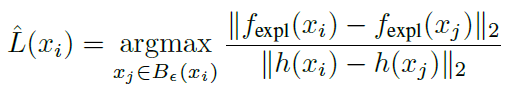
\includegraphics[width=200pt]{figures/stability_metric.PNG}
\end{equation} 

\parencite{barakat2010rule} already commented on the importance of comprehensibility, accuracy and fidelity for rule extraction techniques that explain a SVM model though rule extraction techniques. The metrics are defined as:
\begin{itemize}
    \item \textbf{Accuracy} = Number of instances classified correctly by the rules / Length test set
    \item \textbf{Fidelity} = Number of instances where the rule predictions match the model predictions / Length test
    \item \textbf{Consistency} = Number of of rules and No. of antecedents (analogous to rule size).
\end{itemize}

\parencite{vilone2020comparative} shows a model-agnostic comparative for rule extraction algorithms using C4.5Rule-PANE, REFNE, RxREN and TREPAN. For that, they use 8 data sets of up to 8124 total instances and 40 features. As blackbox models they use Neural Networks models for classification (with different configurations). Finally, they propose several metrics for measuring the quality of the explanations.

\begin{itemize}
    \item \textbf{Completeness:} Percentage of input instances covered by rules over total input instances. Analogous to "Representativeness".
    \item \textbf{Correctness:} Percentage of input instances correctly classified by rules over total input instances. Analogous to "Accuracy".
    \item \textbf{Fidelity:} Percentage of input instances on which the predictions of model and rules agree over total instances.
    \item \textbf{Robustness:} Applying small perturbations over the data points that do not change the prediction of the model, the sum of differences between the original prediction and the new prediction, divided by the number of instances analyzed. It is analogous to the concept of "Stability".
    
    \begin{equation}
    \begin{split}
      Robustness = \frac{\sum_{n=1}^{N} f(x_n) - f(x_n + \delta)}{N} \\
    \end{split}
    \end{equation}
    
    Robustness is further analysed in \parencite{alvarez2018robustness}, where the authors evaluate it for feature relevance model-agnostic post-hoc XAI techniques (LIME and SHAP).
        
    \item \textbf{Number of rules} and \textbf{Average rule length}, similar to \parencite{barakat2010rule}.
\end{itemize}

They apply these metrics and see, using the Friedman's test, that C45-Pane has significantly superior results over all of the data sets considering all of the metrics, followed by TREPAN.

A summary of all these proposal appears in \hyperref[table:ch2-sota-taxonomy-sota]{Table} \ref{table:ch2-sota-taxonomy-sota}, including some direct mappings between them. 

\begin{table}[h!]
\centering
\resizebox{220pt}{!}{%
\begin{tabular}{@{}llllll@{}}
                                                     & \rot{{\parencite{carvalho2019machine}}}
                                                     & \rot{{\parencite{hoffman2018metrics}}}
                                                     & \rot{{\parencite{melis2018towards}}}
                                                     & \rot{{\parencite{barakat2010rule}}} 
                                                     & \rot{{\parencite{vilone2020comparative}}}
                                                     \\ \midrule
\multicolumn{1}{l|}{Accuracy/Correctness}            & X & X &   & X & X \\
\multicolumn{1}{l|}{Fidelity/Faithfulness}           & X &   & X & X & X \\
\multicolumn{1}{l|}{Consistency}                     & X &   &   &   & X \\
\multicolumn{1}{l|}{Stability/Robustness}            & X &   & X & X &   \\
\multicolumn{1}{l|}{Comprehensibility}               & X & X &   & X &   \\
\multicolumn{1}{l|}{Certainty}                       & X &   &   &   &   \\
\multicolumn{1}{l|}{Importance}                      & X &   &   &   &   \\
\multicolumn{1}{l|}{Novelty}                         & X &   &   &   &   \\
\multicolumn{1}{l|}{Representativeness/Completeness} & X &   &   & X &   \\
\multicolumn{1}{l|}{Contrastiveness}                 & X &   &   &   &   \\
\multicolumn{1}{l|}{Selectivity}                     & X &   &   &   &   \\
\multicolumn{1}{l|}{Social}                          & X &   &   &   &   \\
\multicolumn{1}{l|}{Focus on the abnormal}           & X &   &   &   &   \\
\multicolumn{1}{l|}{Truthful}                        & X & X &   &   &   \\
\multicolumn{1}{l|}{Consistent with apriori beliefs} & X &   &   &   &   \\
\multicolumn{1}{l|}{General and probable}            & X &   &   &   &   \\
\multicolumn{1}{l|}{Explicitness}                    &   &   & X &   &   \\
\multicolumn{1}{l|}{Feeling of Satisfaction}         &   & X &   &   &   \\
\multicolumn{1}{l|}{Usefulness}                      &   & X &   &   &   \\
\multicolumn{1}{l|}{Completeness}                    &   & X &   &   &   \\
\multicolumn{1}{l|}{Sufficiency of Detail}           &   & X &   &   &   \\ \bottomrule
\end{tabular}%
}
\caption{Summary of the metric properties for XAI within the referenced literature, including some direct mappings between them.}
\label{table:ch2-sota-taxonomy-sota}
\end{table}


\section{XAI for anomaly detection}\label{sec:ch2-sota-xai-anomaly-detection}
After describing general aspects about XAI, in this section, we focus on the literature regarding XAI and anomaly detection through several aspects. First, we provide an introduction to the specific literature about XAI and anomaly detection, focusing on previous research regarding XAI and OCSVM. Then, we cover another aspect that is relevant for XAI in general, and for XAI for anomaly detection in particular: XAI with prior domain knowledge. 

\subsection{Introduction}\label{subsec:ch2-sota-xai-anomaly-detection-intro}
XAI is useful for both explaining an anomaly detection model from a global perspective, or for explaining the identification of particular instances as outliers. From the global explanation level, \parencite{tallon2020explainable} use two anomaly detection ML algorithms (Decision tree and DeepLog) to detect outliers. Together with that, they use Shapely values in order to generate model-agnostic feature relevance explanations that help to see which features contribute more for predicting outliers by seeing the individual contribution of each feature to the general outlier probability. 

XAI has also been used for anomaly detection for predictive maintenance \parencite{langone2020interpretable}. The authors highlight that even when an anomaly detection model is very accurate, the operators that will get the model prediction may not trust it if it remains a blackbox that does not provide any insights about its decisions. Because of that, they propose an anomaly detection system where the explanations are generated thanks to the usage of a whitebox model (ElasticNet Logistic Regression). So, they provide explanations in terms of feature relevance, focusing on explaining what contributes to an anomalous state. With that, they highlight that explanations for anomaly detection can be generated in a similar way to those of a supervised ML model for binary classification (even though anomaly detection models provide an output heavily imbalanced) 

Shapely values for explaining anomalies are also used at \parencite{mitani2020highly}, where the SHAP algorithm is used to generate feature relevance explanations in order to explain what contributes to specimen mix-up. For the anomaly detection, they use a Gradient Boosting Tree in order to be able to learn efficiently from highly unbalanced data while yielding good predictions. The authors highlight the importance of having a highly accurate model that is able to predict correctly the specimen mix-up, because this is a crucial problem that may lead to an incorrect diagnostic or an inappropriate therapy.

An additional recent reference of XAI for anomaly detection is \parencite{ruff2021unifying}. Their focus on explanations is mainly for unsupervised deep learning (DL) models, where the explanations can be produced by model-agnostic post-hoc techniques for feature relevance (LIME) or by using model specific algorithms (LRP). One of the usages of XAI that they describe is the improvement of the model based on the explanations provided. They show an example for anomaly detection based on images, where XAI helps to see the cases where the pixels used for making the decision are actually the correct ones.

The analysis of the literature highlights how detecting anomalies is critical within some domains, and because of that, their detection needs to be very precise. However, being able to detect anomalies is not enough, and explanations are needed for both understanding the model better (and seeing if it can be trusted or improved), as well as for explaining the model for other audiences in order to see if they can also rely on the predictions or not (something connected to the explanation generation for different user profiles \parencite{arrieta2020explainable}). A model may perform apparently very well and explanations may help to see that the model is taking its decision by using features that are not relevant \parencite{molnar2019interpretable}, so in that case, the model may not be finally trusted. This shows that XAI can complement the classical evaluation of models based only on their performance.

However, after the assessment of a model and seeing that it behaves correctly (from both the XAI and the performance point of view), before providing explanations to some user profiles, it is important to ensure that they are aligned to what the model predicts, and are not showing any contradictory information. One way to accomplish that within the scenario of rule extraction techniques is by using P@1 rules with respect to the model output. Here, the rules may not be explaining all the possible model's outputs, but the explanations will never contradict it.

For feature relevance explanations, the literature shows that they help to see how they contribute to the positive class (outliers in anomaly detection). For rule extraction explanations, they can help to explain outliers with respect to what will turn that outlier into an inlier. Considering this, the explanations will target the inlier class, so the outliers can be explained in a counterfactual approach with respect to the non-anomalous subspace (for local explanations). For global explanations that help to see what feature values are normally associated to outlier situations, the explanations would still target the outlier class.


\subsection{XAI for OCSVM}\label{subsec:ch2-sota-xai-oscvm}
Searching in the Scopus\textsuperscript{\textregistered} \footnote{Last searched in 01/02/2020.} database for titles, abstracts, and/or keywords that contain the terms "XAI", "explainable" or "interpretable", together with "OC-SVM" or "OCSVM", only provided 4 results.

One of them is the work of \parencite{kauffmann2020towards}. Here, the authors propose a model-specific method based on the fact that OCSVM models can be rewritten as pooling neural networks. Due to the asymmetry between inliers and outliers, they model with a min-pooling over distances for outliers, and a max-pooling over similarities for inliers. Thanks to turning OCSVM models to a neural network, they apply a deep Taylor decomposition (DTD) to obtain explanations in terms of input features. DTD serves as a framework to apply layer-wise retropropagation (LRP) in order to obtain the feature contribution of the input features to a predicted output. The authors extend the explanations generated to include using both input features or support vectors. 

In \parencite{itani2020one} the authors benchmark different unsupervised ML algorithms for anomaly detection (IsolationForests, OCSVM, Cluster Support Vector Data Description and One-Class decision Tree, OC-Tree), and analyse them over data from the medical domain. They indicate that OC-Tree provides the best results, with the advantage of being a hybrid method that combines the first kernel density estimation for anomaly detection with a decision tree that automatically provides rules that explains the first model. The benchmark of the models is performed in terms of predictive performance, mentioning that OC-Tree is then better for that use case since it directly provides explanations.

In \parencite{jang2019anomaly} the authors use OCSVM and Variational Autoencoders for detecting engine faults within 2.4L diesel engines. The faults, which may belong to two types, are precisely the anomalies. For that they use 130 feature parameters. Together with that, they include a post-hoc explainability layer by using LIME (thus, explaining the models in terms of feature relevance).

\parencite{padmaja2015hybrid} also shows the combination of OCSVM with XAI. For the XAI part, they use the algorithm Ripper for rule induction. For this algorithm, they use the information from the support vectors from the OCSVM. At the evaluations, they use three different data sets and measure the performance of the rules extracted in terms of Precision, Recall and F1 metrics over the ground truth of the real anomalies. They also train OCSVM models with a RBF kernel.

The previous analysis of the literature shows that even though there are some works regarding XAI and OCSVM, they are either focused in a particular domain, or they do not compare several XAI methods in order to assess their differences (from either a model's performance or explanainability point of view). Due to that, there is still an open area regarding the benchmark of rule extraction techniques over OCSVM models for anomaly detection.

\subsection{Domain knowledge combined with XAI}\label{subsec:ch2-domain-knowledge-xai}
Within the review of \parencite{arrieta2020explainable}, one of the open research challenges is combining domain knowledge with the explanations generated to enhance the user's understandability. This challenge is especially addressed through the combination of deep learning black box models together with symbolic approaches (as covered within the field of neurosymbolic approaches). These last approaches are algorithmic transparent and generally directly interpretable, and with domain knowledge expressed through ontologies. This is the case of \parencite{confalonieritrepan}, where the authors propose a variant of the TREPAN algorithm that uses domain ontologies in the XAI phase. TREPAN uses surrogate decision trees to explain any black box model (model agnostic). However, as the authors highlight, those trees are often not understandable by a final user. That is why they propose a variation on the algorithm that gathers information from a domain ontology and uses it to prioritize using features for the splits that are more general within the ontology. The prioritization is done by penalizing the Information Gain value when considering a feature from the split that is too specific.  They assessed their proposal with expert users in the finance and medical domains, and found that using domain knowledge enhances the user's understandability.

Indeed, domain knowledge can be applied to adjust the explanations generated, and it can be done at different moments during a ML model life cycle. It can be done at the ML model itself (for instance, finding hyperparameters that enhance the model understandability), or during the training of a post-hoc XAI method. Finally, it can be also applied after the XAI method generates the explanations, to adjust them to the existing domain knowledge. This is shown within the literature review of \parencite{beckh2021explainable}. Authors indicate how there are three scenarios regarding XAI and prior domain knowledge. First, mainly for posthoc approaches, integrating the knowledge at the underlying ML level either by combining it with the data set, during the grid search for adjusting the hyperparameters, for defining the cost function, or for postprocessing the output (e.g., for choosing the classification threshold). Second, by integrating the knowledge within the XAI method (with similar sub-approaches as the ones for the integration with the underlying ML method). Finally, they also indicate cases where new knowledge can be derived from the explanations, such as detecting bias problems with the ML model thanks to XAI, or building new applications and use cases thanks to the XAI explanations.

The combination of domain knowledge and XAI is crucial, since this helps preventing the generation of explanations that only explain the model decision in terms of correlations, ignoring any causality aspects, which can led explanations that are false or misleading \parencite{holzinger2019causability}.

\section{Introduction to anomaly detection in real-world contexts}\label{sec:ch2s-sota-specific}
%Within this section, we review the SOTA regarding the factors that impact on the fuel consumption of diesel and petrol vehicles, since this is one of the main use cases studied within this thesis. This analysis is important for eliciting the features for training the ML models, as well as for analysing if the explanations are aligned to that prior domain knowledge. We also review previous literature regarding vehicle fuel prediction with some of these factors using ML, as well as the usage of anomaly detection models for detecting vehicle fuel anomalies.

In this section, we review the SOTA regarding anomaly detection within real-world contexts, particularly for the use cases of Mobile Network Operators (MNO) covered in this thesis: anomaly detection in network communications data, and anomaly detection in vehicle fuel usage. We will describe the context of anomaly detection within these contexts, along with the techniques used related to ML. We will also highlight the features that are normally used for identifying the anomalies in those contexts. This analysis is important for eliciting the features for training the ML models, as well as for analysing if the explanations are aligned to that prior domain knowledge.

\subsection{Anomaly detection in network traffic}\label{subsec:ch2-sota-comms}

% Reviews of anomaly detection in network traffic
The problem of anomaly detection within network traffic is a common use case within MNO since it is crucial within several applications. The review of \parencite{fernandes2019comprehensive} highlights how important it is to detect anomalies in order to avoid significant service degradation, malicious damage or for reducing costs. An anomaly could be considered as a "\textit{observation (or subset of observations) which appears to be inconsistent with the remainder of that set of data}" \parencite{barnett1984outliers}, though it is important having a prior knowledge about the type of anomalies in order to address the problem properly. For traffic anomalies, they classify the literature depending on the nature of the anomalies (point, collective or contextual), or on the causal aspect (operational, flash crowd, measurement,  or network attack). 
Regarding the nature:
\begin{itemize}
\item \textbf{Point anomaly}: A single data point has a different behaviour compared to its data group
\item \textbf{Contextual anomaly}: Data is anomalous within a specific context. This is common within time series, where an anomaly may happen during a specific time interval (but outside it, that same point would not be anomalous).
\item \textbf{Collective anomaly}: A collection of data groups have an anomalous behaviour within the whole data set.
\end{itemize}

This classification of anomalies based on their nature is not specific to network traffic. Nonetheless, the authors also classify the literature based on the causal aspect, specific to network anomalies:
\begin{itemize}
\item \textbf{Operational events}: Server crashes, power outages, traffic congestion, large transfers (non-malicious), inadequate resource configuration.
\item \textbf{Flash crowds}: Legitimate but abnormal use. Large flows in traffic normally caused by a rapid growth of users trying to access a specific network resource (e.g., an e-commerce website announces a promotion and a lot of people access the site simultaneously)
\item \textbf{Measurement anomalies}: Other type of anomalies different from the ones above, and that are also non-malicious. They are related to problems during the data collection phase.
\item \textbf{Network abuse anomalies}: They are malicious attempts to disrupt, deny, degrade or destroy information and services from computer network systems.
\end{itemize}

They also provide a taxonomy based on the techniques used for anomaly detection, which is also something that can be used within other use cases. They classify the literature depending on whether they use evolutionary computation, finite state machine, clustering, information theory, classification, statistical or other techniques.

The review of \parencite{ali2020review} indicates similar taxonomy approach for network anomaly detection, using the same classification for the nature of the anomalies, and providing classification based on the ML techniques used. For this last aspect, they indicate techniques related to supervised classification (SVM, Naive Bayes, Neural Networks, Nearest Neighbours or Decision Trees), semi-supervised learning, or unsupervised learning (mainly related to different types of clustering techniques).

% Anomaly detection in MNO
The work of \parencite{gunavathi2019big} presents a proposal for anomaly detection within Call Detail Records (CDR) data, using unsupervised clustering techniques. They first define a set of features related to the call-in (received calls) and call-out (outgoing calls) information, and then they generate a feature that indicates the activity for that particular CDR. With that and using the clustering techniques, they group the CDRs based on the behaviour, and they use that for finding CDRs that are anomalous based on their activity. Activity could be anomalous either because it is to high or it is too low compared to the normal behavioural pattern.

% Anomaly detection in Call Centers
For the particular case of Call Centers, the work of \parencite{iheme2019feature} presents the usage of OCSVM models for detecting anomalies within the calls in order to detect potential malpractices in the agents. They use several features are used for modelling the calls: call duration, average silence duration, dBFS (loudness of the call), or the percentage of silence, among others.

% Finally, only reference that combines XAI and anomaly detection within a MNO use case
However, even though the literature is extensive in terms of network anomaly detection (and related use cases), there is a lack of research regarding the usage of XAI in these contexts. The only explicit reference for XAI for anomaly detection for network related use cases is, to the best of our knowledge, the recent work of \parencite{irarrazaval2021telecom}. There, authors research anomaly detection on traffic networks to detect traffic pumping. Traffic pumping is a type of fraud that happens in some countries, where a local operator with high access charge rate has an agreement with another one with high call volume operations (which is usually free of charge), so the number of calls into the local operator is stimulated, then sharing a portion of its increased access revenues with the bigger one. For their use case, there are no labels, so they use unsupervised clustering for finding the anomalies. They use then a decision tree using the clustering labels as prediction labels, and they infer rules about each group. These rules are given to telecommunications experts so they can validate them or study the corresponding cluster in more detail, and identify which groups are anomalous. Thus, they do provide a XAI based solution which through a global surrogate post-hoc model (Decision Tree) that explains with rules the relationship between input features and output clustering labels. They also built a set of features that can be easily incorporated in an explanation (an important aspect in order to enhance the understandability aspect \parencite{arrieta2020explainable}).


\subsection{Factors for fuel consumption in a vehicle}\label{subsec:ch2-sota-fuel-factors}
In the previous subsection we indicated how the detection of anomalies in real-world contexts requires the use of prior domain knowledge, and this step is crucial for choosing the set of features for both detecting and explaining these anomalies. Thus, in this subsection, we will analyse in detail the features that may impact on the fuel usage, since it is a field very well researched.

Fuel consumption can significantly vary from one vehicle to another, even when comparing two vehicles from the same make, model, year and fuel type. This is caused by different factors that may increase or decrease the amount of fuel consumed during the same trip. The literature contains many studies that identify these factors and assess how much fuel could be saved when they are optimized. This is something very relevant for fleet managers.

\parencite{zhou2016review} presents a literature review of different factors that have a potential impact in the fuel consumption of a vehicle, together with their relative importance. \hyperref[figure:ch2-sota-chart-factors]{Figure} \ref{figure:ch2-sota-chart-factors} shows the categories of fuel factors considered in that review. 

\begin{figure}[h!]
\centering
 \begin{tabular}{c@{\qquad}c@{\qquad}c}
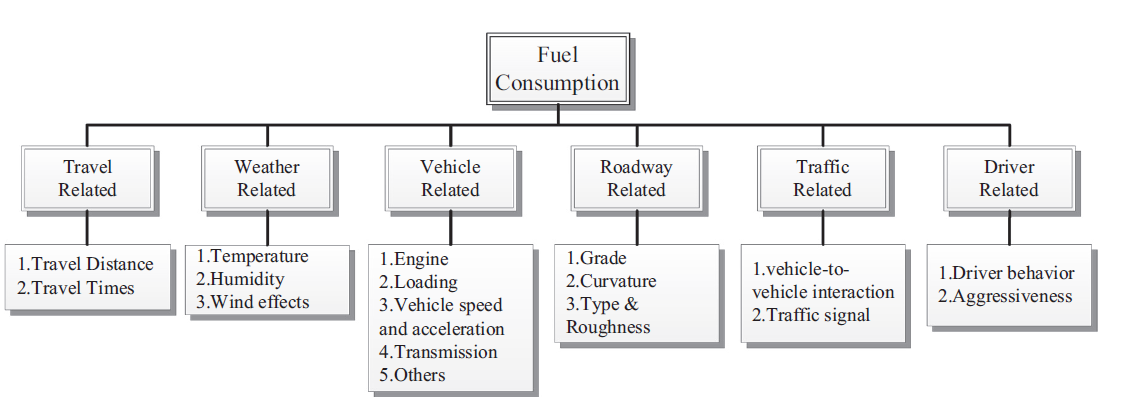
\includegraphics[width=0.8\columnwidth]{figures/chart_factors.PNG}
  \end{tabular} 
  \caption{Categories of fuel factors discussed in \parencite{zhou2016review} \label{figure:ch2-sota-chart-factors}}
\end{figure}

The first category considered are \textbf{travel-related} factors. This group includes factors that are related to the route covered by the vehicle. In fact, the authors mention \textbf{eco-routing} as a crucial aspect to reduce fuel consumption. Fuel can be saved by choosing an optimal route not only in classical terms of distance and travel time, but also in terms of a route that saves fuel compared to other possible ones (e.g.choosing routes with less "bumps" or "slopes"). In fact, the new route may even be longer in time or distance, but offers fuel saving. The paper indicates that eco-routing alone can reduce the fuel consumption of a vehicle by 18\% to 23\%.

The second category includes \textbf{weather-related} factors. These factors impact the fuel consumption of a vehicle in an indirect way (i.e. by being related to the usage of the air conditioner, by affecting the water pump, by increasing the engine or transmission friction in a cold weather...). Thus, this category includes factors like the exterior temperature, the relative humidity or the wind effects. These factors may be responsible for about a 1\% of the fuel consumption of a vehicle.

The third group of factors are named \textbf{vehicle-related}. It includes factors mainly related to the engine and the vehicle itself, such as vehicle load, vehicle speed, engine speed, type of fuel, whether the vehicle has an exhaust after-treatment system or not... 

The fourth group is named \textbf{roadway-related factors}. It refers to factors related to the road condition, like the road slope, the surface roughness, or the road curvature. These factors, though not being very actionable (sometimes it is difficult to prevent them), have a large impact on the fuel consumption (around 5 to 20\%).

The fifth group of factors refer to \textbf{traffic conditions}. They are very related to a good arrangement of traffic signs, such as traffic lights. They have the potentially biggest fuel impact (around 22 to 50\% of the fuel consumption).

Finally, the sixth group mentioned in the review are the \textbf{driver-related} factors, like the driving behaviour or the aggressiveness of the driving. The driving profile of a particular driver (that measures aspects such as that driving aggressiveness), are calculated with vehicle information such as the RPM (engine speed; revolutions per minute), the speed or the acceleration. The authors mention how aggressive driving can be responsible for up to 40\% of the fuel consumption of a vehicle when compared to a calmer driving style. 

The aforementioned literature review is enhanced by the study of \parencite{zacharof2016review}. Here the authors present a thorough analysis regarding the influence of different factors for fuel consumption in a vehicle, along with the influence on CO2 emissions. This study considers passenger vehicles under real-world operating conditions. Regarding fuel consumption specifically, the authors offer a summarized view of the literature showing different categories of variables and their proportional impact in the fuel consumption of a vehicle. 

There are two approaches for analysing the impact of a specific factor in the fuel consumption of a vehicle. First, using a simulation analysis that studies the isolated impact of a factor under laboratory conditions. Second, by analysing feeds of data that contain the instant fuel consumption reported during trips on real-world environments. These feeds of data can be gathered from sources such as OBD-II (On-board diagnostics) port \parencite{ISO14230} (e.g. the Engine Fuel Rate with the PID 015E). 

The analysis of the literature highlights that both approaches offer in general similar results (when there are publications available for a specific factor both from the simulation point of view, as well as with the real-world data). Thus, real-world collected data can be a valid data source for assessing the impact of different factors in the fuel consumption of a vehicle.

Here, the literature review proposes a fuel factor taxonomy that in some cases matches directly the one proposed in \parencite{zhou2016review}, but in some others is different. There are 28 factors that can be classified into 9 groups. All these factors, as reported by \parencite{zacharof2016review}, appear at \hyperref[table:ch2-sota-factors-table]{Table} \ref{table:ch2-sota-factors-table}. This Table shows the relative importance of each of the factors (literature median value) along with an interval that encloses the different values reported, considering vehicles under real-world operating conditions. It also shows how many papers talk about that particular factor, as well as the distribution of the relative values reported. 

\begin{sidewaysfigure}[h!]
  \centering
  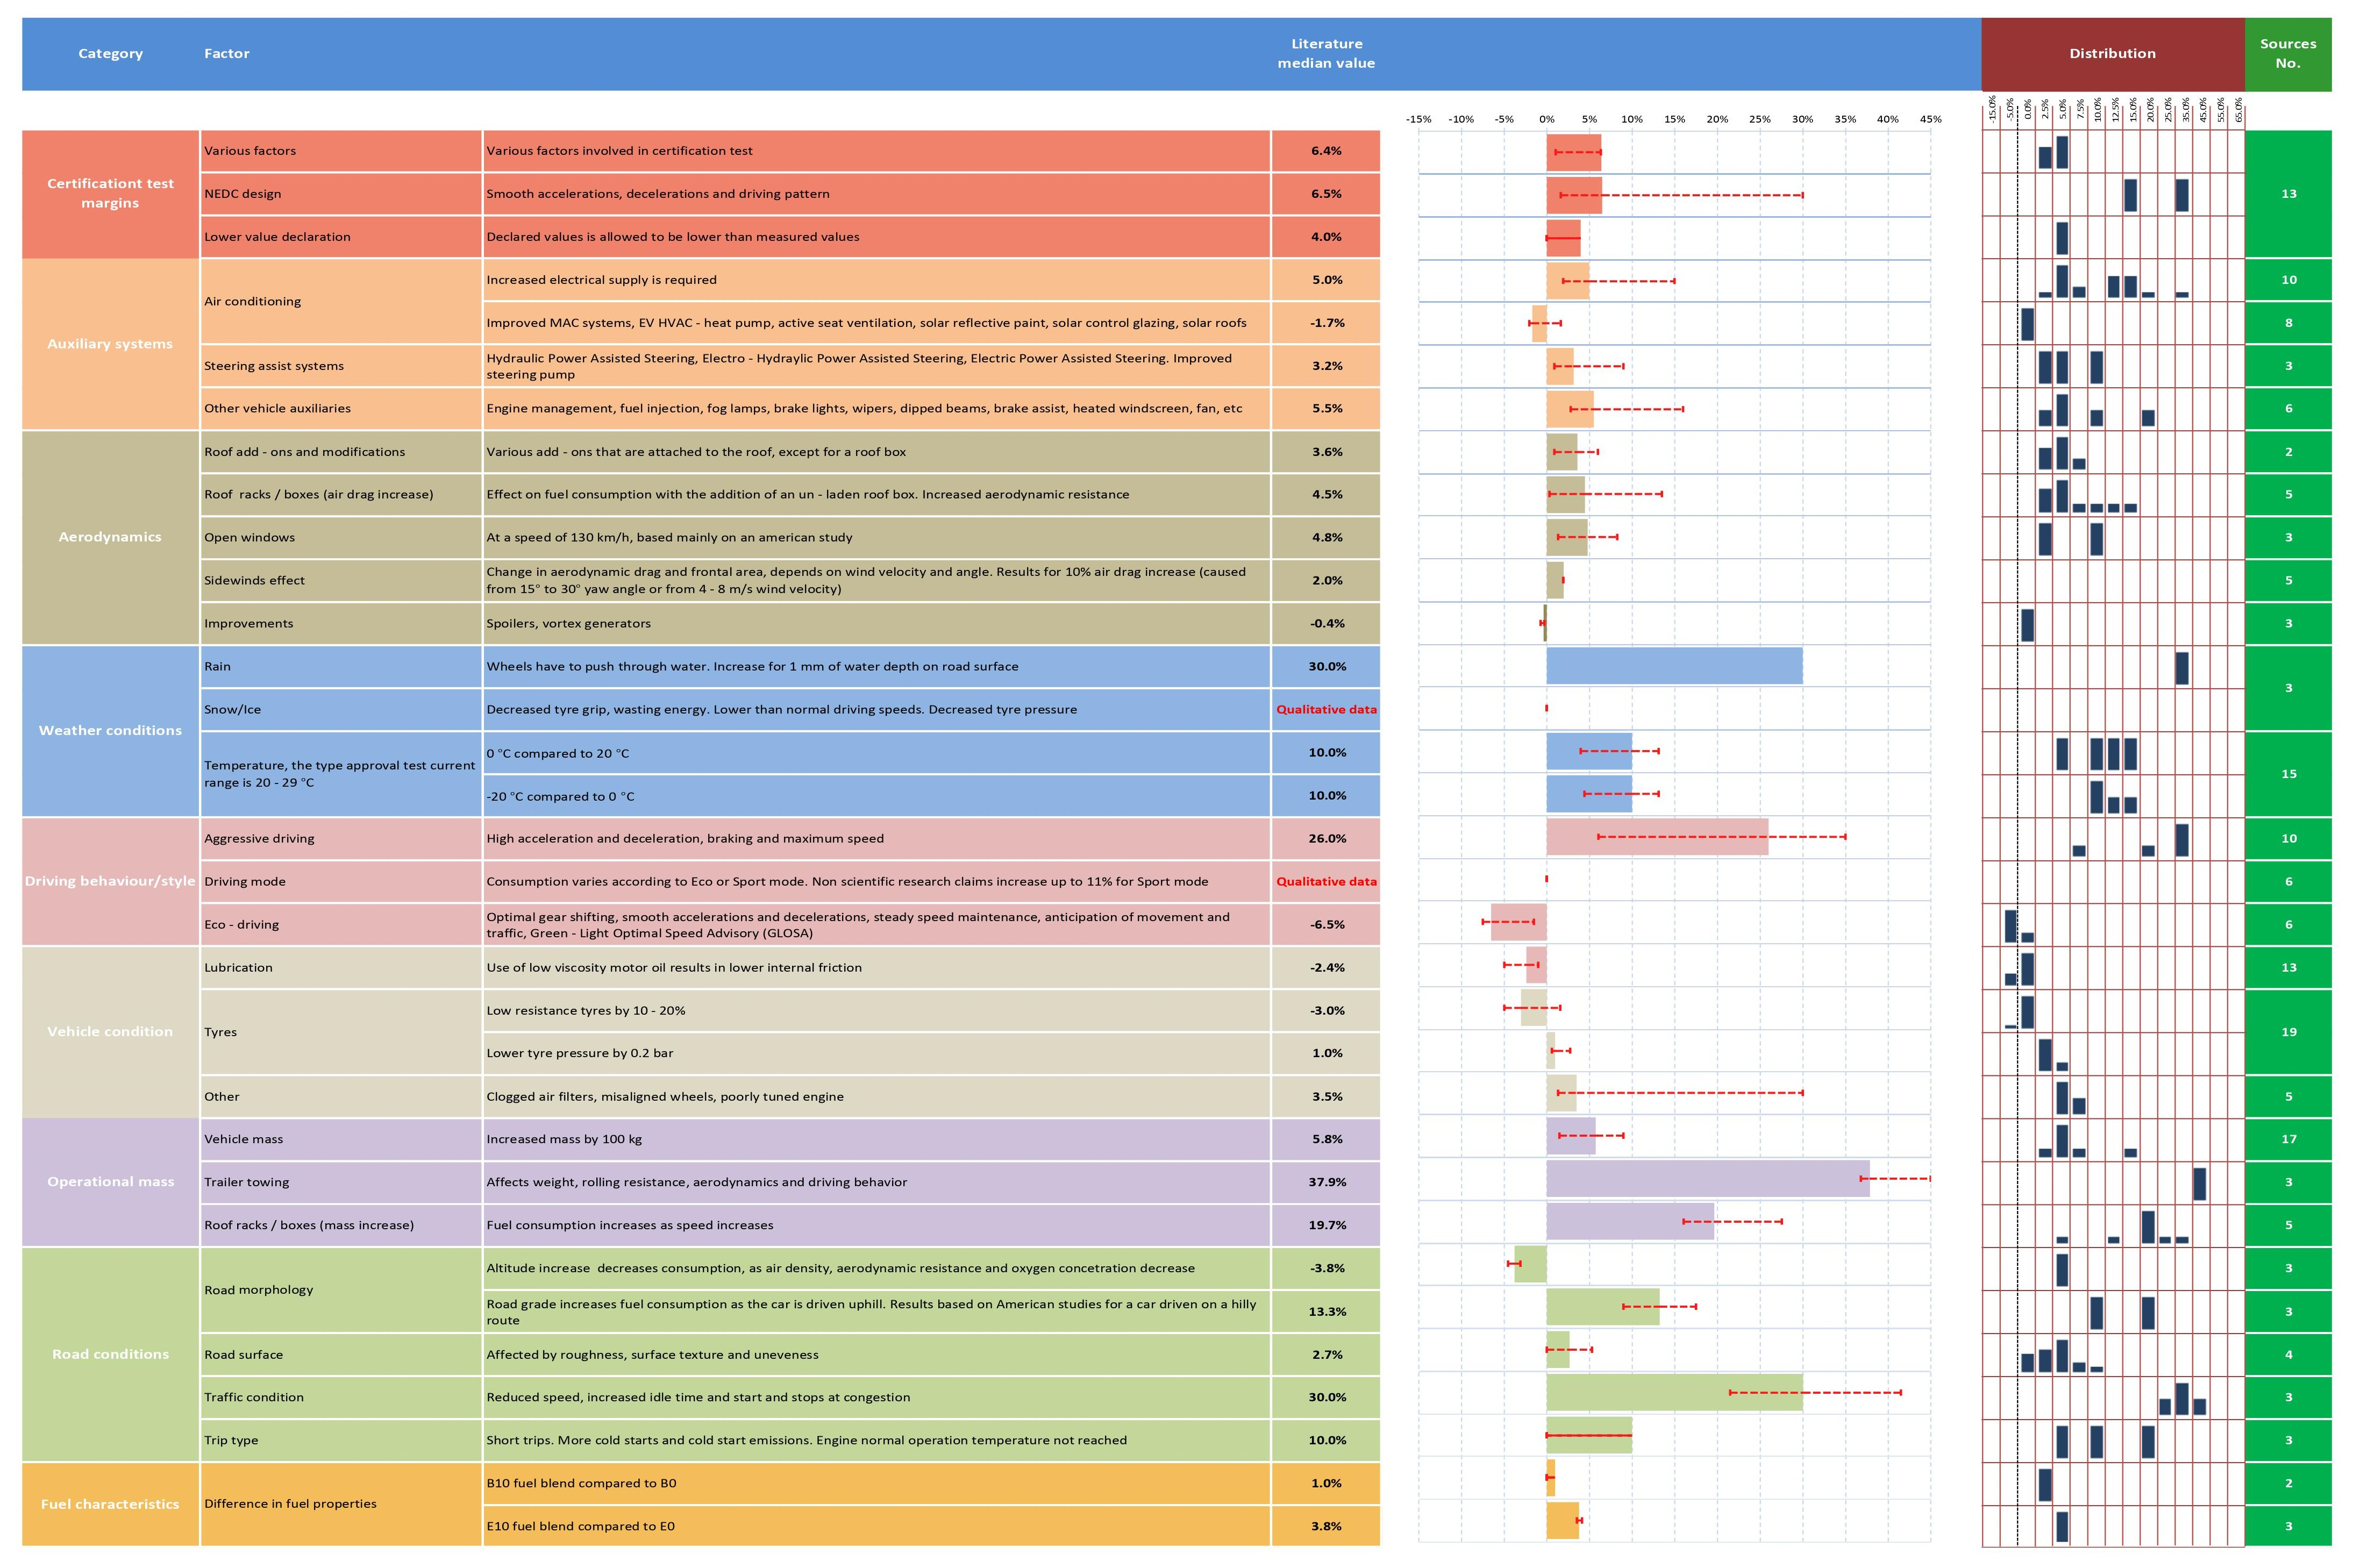
\includegraphics[width=0.95\columnwidth]{figures/factors_table.jpg}
  \caption{Fuel factors mentioned in the literature, together with the relative importance as reported by \parencite{zacharof2016review}}
  \label{table:ch2-sota-factors-table}
\end{sidewaysfigure}

Regarding driver-related factors, \hyperref[table:ch2-sota-factors-table]{Table} \ref{table:ch2-sota-factors-table} shows a group called \textbf{driving behaviour/style} that accounts for factors related directly to the driver. It is almost similar to the one from \hyperref[figure:ch2-sota-chart-factors]{Figure} \ref{figure:ch2-sota-chart-factors} with the exception of considering factors related to good driving styles that may reduce the fuel consumption.

Regarding the group \textbf{road conditions} in \parencite{zhou2016review}, it mainly includes the travel related, traffic related and roadway related factors.

Vehicle-related is the group with more factor's differences between both papers. Compared to \parencite{zhou2016review}, these factors are split into \textbf{auxiliary systems}, \textbf{vehicle conditions} and \textbf{fuel characteristics}, complemented with other groups that include factors related to the vehicle's design itself (\textbf{aerodynamics} and \textbf{operational mass}) and to \textbf{certification test margins}. In this last review, all these vehicle-related factors account for aspects related to the vehicle itself, not considering anything directly related to the driver. This is a difference when compared to the taxonomy of \parencite{zhou2016review}, because vehicle-related includes acceleration and speed factors.

The difference between the analyses shown in both articles are not only in terms of the taxonomy proposed to group factors, but sometimes also regarding the reported impact (i.e. exterior temperature has a median impact reported value of 10\% at \parencite{zacharof2016review} against the 1\% impact for all weather related causes reported by \parencite{zhou2016review}).

Within this last taxonomy of features that affect the fuel usage of a vehicle, some of them could be considered as "actionable", thus, they could be changed in a particular vehicle; in some cases without even needing to change the vehicle's route. An example of this is the aggressive driving style. Other features are inherent to the vehicle and cannot be directly changed, like the vehicle make/model or the vehicle mass. Even within the "actionable" features, some of them cannot be easily read through OBD-II (e.g., if there are roof add-on, which affects the vehicle aerodynamics). Thus, a subset of these features that considers only the ones that are "actionable" and the ones that can be read is the one shown in \hyperref[table:ch2-sota-FeatureInfluenceReduced]{Table} \ref{table:ch2-sota-FeatureInfluenceReduced}.

\begin{table}[]
\centering
 \begin{tabular}{c@{\qquad}c@{\qquad}c}
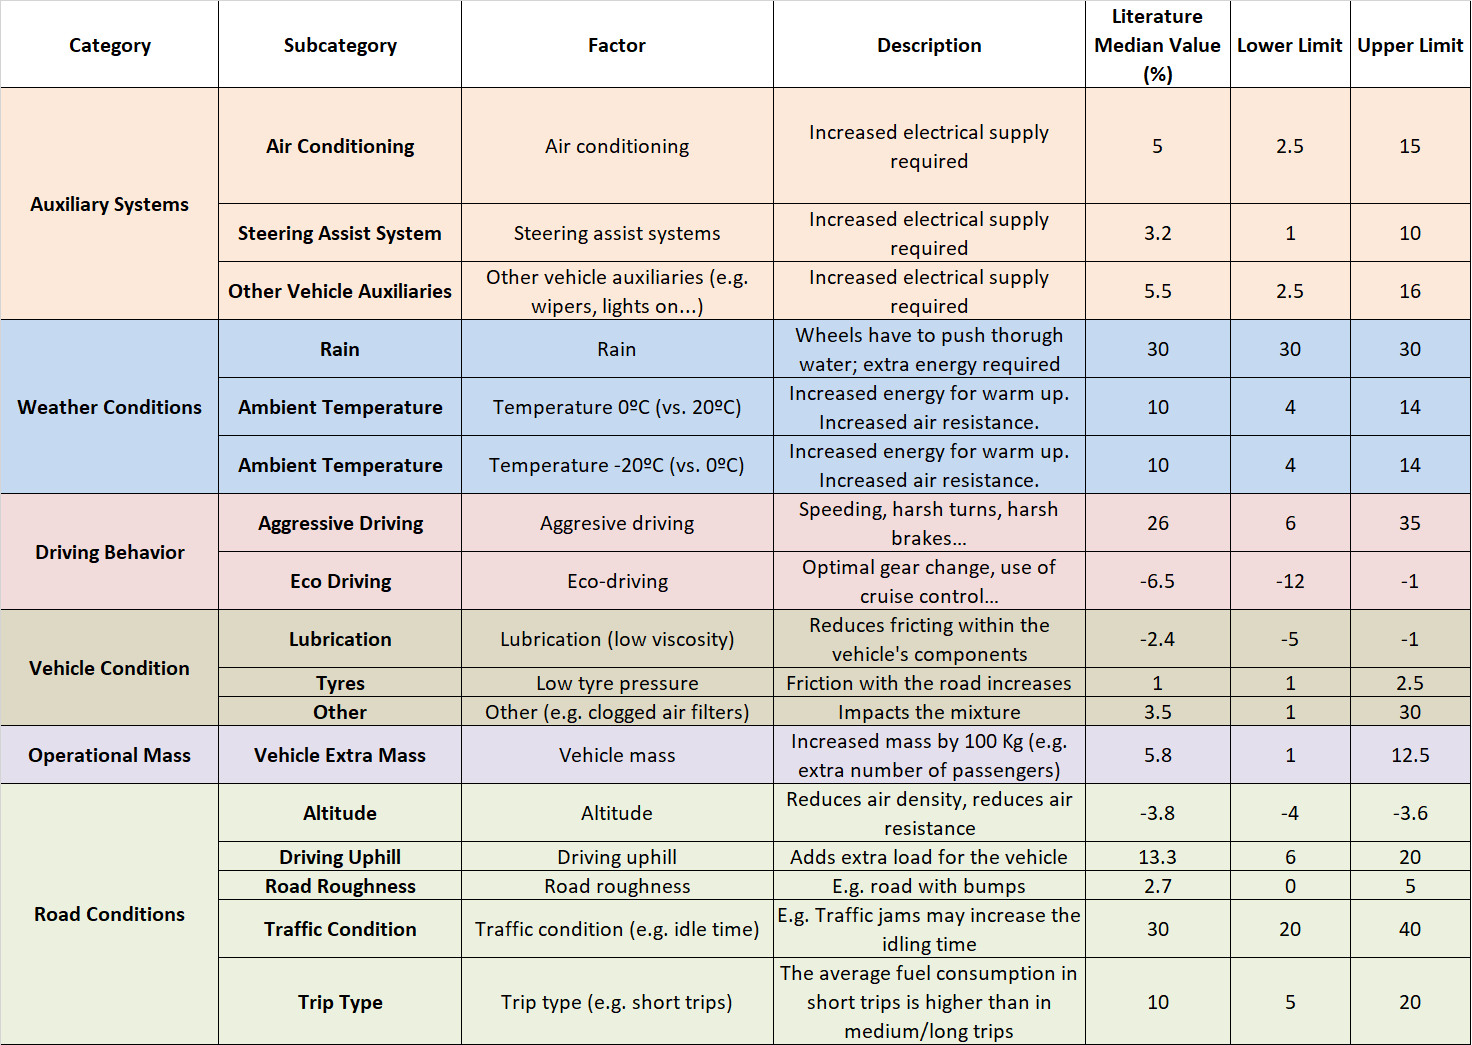
\includegraphics[width=0.90\columnwidth]{figures/FeatureInfluenceReduced.png}
  \end{tabular} 
  \caption{Reduced view from the factors of \parencite{zacharof2016review}, focusing on some of the actionable variables that can be retrieved from the OBD-II. The upper and lower limits refers to the minimum and maximum SOTA values reported in the review. For Rain, the lower limit is set to zero since the review does not provide limits for that feature. \label{table:ch2-sota-FeatureInfluenceReduced}}
\end{table}

The physical reasons as to why these features impact the fuel usage are:
\begin{itemize}
\item \textbf{Air conditioning (A/C)}: Using A/C increases the energy supply needed, leading to an increased fuel consumption. The time using the A/C and the power needed will increase/decrease that extra energy required. This category also includes the heating systems and related features, like the vehicle's coolant.
\item \textbf{Steering assist system}: These systems help driving safely and more confortable, but require additional electrical supply in exchange. An example is the usage of Electric power assisted steering (EPAS).
\item \textbf{Other vehicle auxiliaries}: These features include other auxiliary elements of the vehicle that may also require an extra energy. An example is the vehicle lights usage, that require extra energy and due to that, extra fuel.
\item \textbf{Rain}: Rain (and snow) impact the fuel usage in different ways. First, they affect the wheel gripping to the road surface. Also, the wheels have to push through an additional layer of water (or snow), so extra energy is required.
\item \textbf{Ambient temperature}: Temperature affects tyres, motor oil viscosity, cold start engine… Extra fuel is required in low temperatures to warm up the engine. It also affects aerodynamics: increased air density and higher aerodynamics resistances.
\item \textbf{Aggressive driving}: Aggressive driving is shown through different variables: acceleration patterns, gear change, harsh turns, harsh brakes, speeding... The impact on the fuel usage could be high.
\item \textbf{Eco driving}: Eco driving is related to the optimal driving of a vehicle, which may reduce its fuel usage. It involves optimizing the gear shifting (related to the usage of cruise control), choosing the best possible route thanks to a navigation device...
\item \textbf{Lubrication}: Overcoming of friction within the vehicle's components requires energy, and this is related to the fuel usage. If the friction is minimized thanks to an adequate lubrication, the energy required will be lower.
\item \textbf{Tyres}: Tyre pressure is related to the rolling resistance coefficient (RRC). When the tyres have low pressure, the contact surface with the road increases and more energy is needed to rotate the wheel (as the friction increases). 
\item \textbf{Other (vehicle condition)}: Beside tyres and lubricants, there are other vehicle conditions that impact the fuel usage. For instance, if the air filters are clogged. This is something that happens mainly in old models (since fuel injection in new cars is adjusted to ensure the correct mixture). Other examples are misaligned wheels and suspension losses. 
\item \textbf{Vehicle extra mass}: Extra mass in a vehicle (measured, for instance, in additional 100Kg), increase the energy needed to move the vehicle. This may happen for instance when there are additional passengers in a vehicle.
\item \textbf{Altitude}: In higher altitudes the air density is lower, so the air resistance that the vehicle faces while driving is also lower. This means that in higher altitudes the vehicle needs lower energy to move the same distance.
\item \textbf{Driving uphill}: Driving uphill adds an extra load over the vehicle, that needs additional energy to move. By contrast, driving downhill reduces the amount of energy needed.
\item \textbf{Road roughness}: For instance, if a road has many bumps, the vehicle will need additional energy to go through it. 
\item \textbf{Traffic condition}: Traffic condition also impacts in the fuel usage. For instance, if there are traffic jams, the idling time normally increases, leading to an increased average fuel consumption.
\item \textbf{Trip type}: The trip type also impacts in the fuel usage. For instance, if the trip distance is small, the average fuel consumption will increase, since fuel is required to turn on the vehicle.
\end{itemize}

There are some additional factors that impact in the fuel consumption that the previous references did not mention. This is the case of Diesel Exhaust Fluid (DEF). DEF is an urea-based product used in after-treatment processes of the vehicle, such as Selective Catalytic Reduction (SCR). It is applied over the vehicle's exhaust stream in order to transform the NOx gas emissions into nitrogen, water and CO2, reducing the NOx emissions in the process \parencite{betageri2016effects}. Techniques like SCR do not only reduce the emissions of a vehicle, but also help the engine performance and may lower fuel consumption \parencite{chen2015nonlinear, chen2013integrated}.

The factors already mentioned are linked to passenger vehicles, but for other vehicles, such as trucks, there are additional ones to consider. This is the case of power take-off, where there is power from the engine that is taken out (e.g. with a splined drive shaft) and used in another application (e.g. for a cement mixer in a truck). This directly impacts in the mileage of a vehicle \parencite{boriboonsomsin2010analysis}.

All these references show that there is a physical and empirically measured connection between the value of specific factors and the value of the fuel consumption. Thus, it is possible to use them in order to predict the value of the fuel consumption with ML models, as already shown within the literature \parencite{9072728, 8727915, perrotta2017application}.

\subsection{Machine Learning for connecting input features to vehicle fuel consumption}\label{subsec:ch2-sota-ml-fuel-consumption}
As we mentioned in the previous subsection, there are several features that affect the fuel consumption of a vehicle. This can be assessed using as input data source the feeds of data gathered from the vehicle's movement together with Machine Learning (ML) algorithms. This is the case of \parencite{ping2019impact}, where the authors conduct a study over a fleet of vehicles where they assess the impact of driving behaviour in the fuel consumption. They consider features related to driving behaviour, such as the gas pedal position, the speed and speed variance, or the steering angle, and they first see how those features have significant correlations with the fuel consumption. Then, they use several clustering algorithms (Spectral clustering, KFCM, K-Means), finding different clusters based on the driver consumption profile and its relationship with those driving behaviour features. 

In \parencite{perrotta2017application}, the authors analyse the impact of other features for fuel consumption within the context of trucks. The 56 features used include characteristics from the vehicle, such as its gross weight, together with others belonging to driving behaviour (usage of cruise control, average speed...), as well as information from the road (like the road surface macrotexture, or the curvature of the road). Those input features are seen as correlated with the fuel consumption (using a bivariate correlation analysis), and then are used to train several ML models (ANN, SVM, Random Forest) in order to predict the fuel consumption of the trucks. For the case of Random Forest, the authors viewed the relative impact from the different features in the fuel consumption through their contribution for accuracy during the tree splitting process.

The previous approaches are useful for detecting dependencies between a set of features and the fuel consumption of a vehicle. However, they do not quantify exactly how many extra liters of fuel are spent due to those features. In \parencite{andrieu2014evaluation}, the authors investigate the impact of eco-driving in the fuel consumption. Eco-driving is expressed through several features related to variables such as the Revolutions Per Minute (RPM) or the braking. Then, they use statistical tests for detecting significant decreases in fuel consumption when an eco-routing driving style is used. Then, they use a Logistic Regression model for analysing the relationship between driver-related features and the fact that the vehicle trip was actually done with eco-routing.

It is possible to use a Linear Regression model for measuring the individual impact of input features in fuel consumption, and know exactly how many liters are used due to each individual variable. The reason behind this is that those models are known as whitebox because they directly provide the influence of the input in the output \parencite{arrieta2020explainable}.
This is shown in \parencite{pavlovic2020understanding}, where the authors predict the fuel consumption gap between type-approval tests and real-world driving trips, using the information of one vehicle during one year, and with 20 different drivers. With that, they build a multiple linear regression model that takes into account driver-related factors as well as environmental and traffic factors in order to predict the fuel consumption gap. Through these linear models, they provide the relative importance for each of the features in the fuel consumption, as well as the r2 value for each of the models tested in order to evaluate them. Similarly, in  \parencite{lasocki2019environmental} the authors study the impact on the fuel of several features inferred related to driving behaviour through the analysis of the data from two different vehicles. One of these features is the Driving Style Indicator (DSI), which is the difference between the average positive acceleration of a vehicle minus the average of the negative acceleration divided by the average speed. The relationship between these features and fuel consumption is modeled through linear regression algorithms in order to quantify the impact of each one of them.

Even though linear regression models can be used for fuel prediction when there is a need of a whitebox ML algorithm that explains the relationship between input and output, this limits the results since the relationship inferred is linear. This problem can be solved by using non-linear whitebox models, such as Generative Additive Models (GAM). However, there is no literature to the best of our knowledge regarding the usage of these models for predicting vehicle fuel consumption.

\subsection{Anomaly detection for fuel consumption}\label{subsec:ch2-sota-anomaly-fuel}
The detection of anomalous fuel consumption in vehicles from a fleet is present at different research works within the literature. In \parencite{aquize2017self}, the authors show how to detect fuel anomalies using unsupervised algorithms (Self-Organizing Maps, SOM). The authors aim to find fuel fraud situations within fleet vehicle data at Bolivia (using a data set of 1000 vehicles with 190627 data points). These situations are normally linked to high fuel purchases within a short period of time. They effectively show how to find clusters within the space of the SOM to identify fuel anomalies and detect fraudulent scenarios by evaluating their proposal over a test set. As the authors mention, there are many features that can be used to contextualize the fuel consumption (e.g., the normal monthly consumption of the vehicle, the behaviour of other vehicles of the same subgroup...). Their proposal leads only to an output that identifies anomalies, but it could be greatly enhanced with XAI techniques that provide additional insights on what contextual features are relevant for that high fuel consumption.

Fuel fraud is not the only case of possible fuel anomalies within a fleet. As described in \parencite{zhang2017safedrive}, driving behaviour may also lead to an increased fuel consumption. Within driving behaviour variables, they mention several features, such as RPM speed, acceleration (both forward, and negative from braking), over speed or gear position.

Even though the previous literature includes research related to the detection of anomalous fuel consumption (both from fraud scenarios and from contextual variables), to the best of our knowledge there are no previous works regarding the explanation of those anomalies using XAI techniques.

\section{Summary}\label{sec:ch2-sota-summary}
In this chapter, we have seen the SOTA regarding XAI and unsupervised ML for anomaly detection, as well as XAI metrics for measuring the quality of explanations, and the combination of XAI with prior domain knowledge. We have also seen the SOTA for the use cases of this thesis: anomaly detection in network traffic, fuel factors that impact on the fuel consumption of petrol and diesel vehicles, and the usage of ML for either predicting fuel consumption or for detecting fuel consumption anomalies.

% Falta de evaluacion de XAI (con metricas) para el caso de modelos de deteccion de anomalias
Within our SOTA review, we detected a generalized lack of research regarding the evaluation of XAI explanations applied within the case of unsupervised anomaly detection. Indeed, the field of XAI metrics itself is still being actively researched, and most of the empirical studies regarding them focus on XAI for supervised ML models for classification and regression tasks, but not for unsupervised ML for anomaly detection, which is a very different task. 

% En el caso de stability/robustness, por ejemplo, solo hay propuestas para feature relevance pero no para rule extraction
% Metricas que faltan XAI
We also saw how even though there are several aspects that XAI metrics should measure (according to different taxonomies), the literature does not provide algorithms for measuring them. For some metrics, like \textbf{stability/robustness}, we saw that previous literature proposes metrics for feature relevance-based XAI techniques. However, there are no proposals, to the best of our knowledge, for other XAI techniques, such as rule extraction. Something similar happens with \textbf{diversity}, a metric which does not have any algorithmic implementation for XAI as far as we know.

% Falta de análisis del uso de domain knowledge con XAI en deteccion de anomalias para ajustar y evaluar las explicaciones, por lo que tiene sentido estudiarlo en un caso de uso real con el caso de fuel consumption.
The SOTA also indicates that even though XAI is useful for generating explanations about a model's decision, the explanations do not normally take into account causality aspects, so they can be misleading or directly incorrect. This is why combining XAI and prior domain knowledge is an important line of research for improving the quality and usefulness of explanations. However, this area is still relatively new, and there is no prior work as far as we know regarding anomaly detection within real-world contexts.

% Y mas metricas en este caso, como monotonicity degree
Related to that, the SOTA also shows that there is a need of XAI metrics that serve to not only compare techniques among themselves (like the aforementioned examples), but also against prior domain knowledge.

\newpage